\documentclass[10pt,aspectratio=43,mathserif,table]{beamer} 
%  设置为 Beamer 文档类型,设置字体为 10pt,长宽比为16:9,数学字体为 serif 风格
\batchmode
\usepackage{graphicx}
\usepackage{subfigure}
\usepackage{fontspec}

% \setmainfont{Harding Text Web Regular Regular.ttf}
\usepackage{diagbox} % 表头斜线分区
\usepackage{unicode-math}
\usefonttheme{serif}
% \setmathrm{Harding Text Web Regular Regular.ttf} % 设置数学字体为 Times New Roman
\setmathfont{TeX Gyre Termes Math} % 如果您使用 XeLaTeX 或 LuaLaTeX 编译,可以使用其他数学字体
\setmathtt{Courier New} % 设置等宽字体为 Courier New
\setboldmathrm{Times New Roman}
\setmathfont{TeX Gyre Termes Math}[version=bold] % 设置粗体数学字体
\setmathfont{TeX Gyre Termes Math}[range={\mathit}]


\usetheme{Berlin} %主题
\setbeamertemplate{page number in head/foot}[pagenumber]
%\usecolortheme{sustech} %主题颜色

\usepackage[ruled,linesnumbered]{algorithm2e}

\usepackage{fancybox}
\usepackage{xcolor}
\usepackage{listings}

\usepackage{booktabs}
\usepackage{colortbl}

\newcommand{\Console}{Console}
\lstset{ %
	backgroundcolor=\color{white},   % choose the background color
	basicstyle=\footnotesize\rmfamily,     % size of fonts used for the code
	columns=fullflexible,
	breaklines=true,                 % automatic line breaking only at whitespace
	captionpos=b,                    % sets the caption-position to bottom
	tabsize=4,
	commentstyle=\color{mygreen},    % comment style
	escapeinside={\%*}{*)},          % if you want to add LaTeX within your code
	keywordstyle=\color{blue},       % keyword style
	stringstyle=\color{mymauve}\ttfamily,     % string literal style
	numbers=left, 
	%	frame=single,
	rulesepcolor=\color{red!20!green!20!blue!20},
	% identifierstyle=\color{red},
	language=c
}


\definecolor{mygreen}{rgb}{0,0.6,0}
\definecolor{mymauve}{rgb}{0.58,0,0.82}
\definecolor{mygray}{gray}{.9}
\definecolor{mypink}{rgb}{.99,.91,.95}
\definecolor{mycyan}{cmyk}{.3,0,0,0}

%题目,作者,学校,日期
\title{Paper Reading}
%\subtitle{\fontsize{9pt}{14pt}\textbf{跨临界分岔}}
\author{Speaker: Yichen Lu\quad \newline  \newline \quad }
\institute{\fontsize{8pt}{14pt}}
\date{\today}
\newcommand{\concept}{Paper Reading}

%学校Logo
%\pgfdeclareimage[height=0.5cm]{sustech-logo}{sustech-logo.pdf}
%\logo{\pgfuseimage{sustech-logo}\hspace*{0.3cm}}

\AtBeginSection[]
{
	\begin{frame}<beamer>
	\frametitle{\textbf{Contents}}
	\tableofcontents[currentsection]
\end{frame}
}
% \beamerdefaultoverlayspecification{<+->}
% -----------------------------------------------------------------------------
\begin{document}
% -----------------------------------------------------------------------------
% \frame{\titlepage}
\begin{frame}
    \begin{figure}
        \centering
        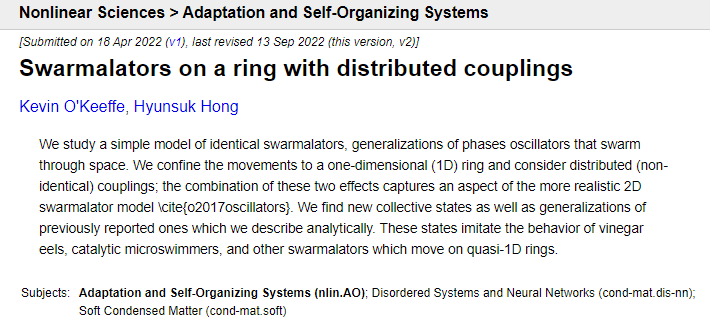
\includegraphics[width=\textwidth]{title.png}
    \end{figure}
    % 手性:swarmalators具有固定的圆形轨道,这个方向可以是顺时针也可以是逆时针
\end{frame}

\begin{frame}
    Model equations:
    $$
    \dot{x}_i=\omega +\frac{1}{N}\sum_j^N{J_j\sin \left( x_j-x_i \right) \cos \left( \theta _j-\theta _i \right)}
    $$
    $$
    \dot{\theta}_i=\nu +\frac{1}{N}\sum_j^N{K_j\sin \left( \theta _j-\theta _i \right) \cos \left( x_j-x_i \right)}
    $$

    Order parameters:
    $$
    W_{\pm}=S_{\pm}e^{i\Phi \pm}\equiv \frac{1}{N}\sum_{j=1}^N{e^{i\left( x_j+\theta _i \right)}}
    $$
    $$
    V=\frac{1}{N}\sum_{j=1}^N{\left< \sqrt{\dot{x}_{j}^{2}+\dot{\theta}_{j}^{2}} \right> _t}
    $$
    'Double delta' distribution
    $$
    \begin{array}{l}
        g\left( J \right) =\delta \left( J-1 \right)\\
        h\left( K \right) =p\delta \left( K-K_p \right) +\left( 1-p \right) \delta \left( K-K_n \right)\\
    \end{array}
    $$


\end{frame}

\begin{frame}
    % \begin{figure}
    %     \centering
    %     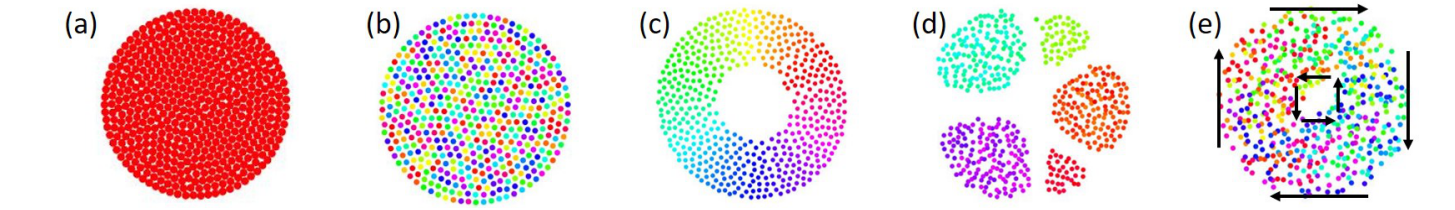
\includegraphics[width=\textwidth]{fig2.png}
    % \end{figure}
    \begin{itemize}
        \item \textbf{Static sync} for $p > p_c$, Order parameters are $S_\pm = 1$ and $V = 0$
        \item \textbf{Static phase wave} for $p_0 < p < p_c$: $x_i = \theta_i \pm C$, $(S_+, S_-) = (1, 0)$ or $(0, 1)$
        % (the $\pm$ refers to a clockwise or counter-clockwise phase wave). 
        \item \textbf{Buckled phase wave} near $p_c$:  A static phase wave
        with a 'buckle', so $S_+ \approx 1, S_-=0, V=0$, which means $x_i \rightarrow \theta_i + C$, $x_i$ and $-\theta_i$ are uncorrelated.
        \item \textbf{Noisy phase wave} for $p < p_0$
        \item \textbf{Async} for $p \approx 0$
    \end{itemize}
\end{frame}

\begin{frame}{Static sync}
    $$
    \left[ \begin{array}{c}
        \dot{x}_i\\
        \dot{\theta}_i\\
    \end{array} \right] =M\left[ \begin{array}{c}
        x_i\\
        \theta _i\\
    \end{array} \right] 
    $$
    where the Jacobian M for the static sync at this fixed point has a block structure:
    $$
    M=\frac{1}{N}\left[ \begin{matrix}
        A&		0\\
        0&		B\\
    \end{matrix} \right] 
    $$
    where 
    $$
    A:=\left[ \begin{matrix}
        -\sum{_{j\ne 1}J_j}&		J_2&		\cdots&		J_N\\
        J_1&		-\sum{_{j\ne 2}J_j}&		\cdots&		J_N\\
        \vdots&		\vdots&		\,\,&		\vdots\\
        J_1&		J_2&		\cdots&		-\sum{_{j\ne N}J_j}\\
    \end{matrix} \right] 
    $$
    
\end{frame}

\begin{frame}
    $$
    A:=\left[ \begin{matrix}
        -\sum{_{j\ne 1}J_j}&		J_2&		\cdots&		J_N\\
        J_1&		-\sum{_{j\ne 2}J_j}&		\cdots&		J_N\\
        \vdots&		\vdots&		\,\,&		\vdots\\
        J_1&		J_2&		\cdots&		-\sum{_{j\ne N}J_j}\\
    \end{matrix} \right] 
    $$
    Sync: 
    $$
    \begin{aligned}
        y_i&=\omega +\frac{1}{N}\sum_j^N{J_j\sin \left( x_j-x_i \right) \cos \left( \theta _j-\theta _i \right)}\\
        &=\frac{1}{N}\sum_j^N{J_j\sin \left( x_j-x_i \right) \,\,  \left( sync\Longrightarrow \theta _j-\theta _i=0 \right)}\\
    \end{aligned}
    $$
    Static: 
    $$
    \begin{array}{r}
        Static\Longrightarrow y_i=0\Longrightarrow \sin \left( x_j-x_i \right) =0\\
        \Longrightarrow \cos \left( x_j-x_i \right) =1\\
    \end{array}
    $$
    $$
    \frac{\partial y_i}{\partial x_i}=-\frac{1}{N}\sum_j^N{J_j\cos \left( x_j-x_i \right)}=-\frac{1}{N}\sum_j^N{J_j}
    $$

\end{frame}

\begin{frame}
    $$
    A:=\left[ \begin{matrix}
        J_1&		J_2&		\cdots&		J_N\\
        J_1&		J_2&		\cdots&		J_N\\
        \vdots&		\vdots&		\,\,&		\vdots\\
        J_1&		J_2&		\cdots&		J_N\\
    \end{matrix} \right] +\left[ \begin{matrix}
        -\left< J \right>&		0&		\cdots&		0\\
        0&		-\left< J \right>&		\cdots&		0\\
        \vdots&		\vdots&		\,\,&		\vdots\\
        0&		0&		\cdots&		-\left< J \right>\\
    \end{matrix} \right] = A_1 + A_2
    $$
    
    $$
    \lambda _{A_1}=0,\left< J \right> , \lambda _{A_2}=-\left< J \right> 
    $$
    Two matrices have the same eigenvector:
    $$
    \left[ \begin{matrix}
        1&		1&		\cdots&		1\\
    \end{matrix} \right] ^T
    $$    
    So $\lambda_A = \lambda _{A_1} + \lambda _{A_2}$
    $$
    \begin{matrix}
        \lambda _{A,1}=0&		\left( \mathrm{w}.\mathrm{m}.\  1 \right)\\
        \lambda _{A,2}=-\left< J \right>&		\left( \mathrm{w}.\mathrm{m}.\  N-1 \right)\\
    \end{matrix}
    $$

\end{frame}

\begin{frame}
    Putting this together gives
    $$
    \begin{matrix}
        \lambda _0=0&		\left( \mathrm{w}.\mathrm{m}. 2 \right)\\
        \lambda _1=-\left< J \right>&		\left( \mathrm{w}.\mathrm{m}. N-1 \right)\\
        \lambda _2=-\left< K \right>&		\left( \mathrm{w}.\mathrm{m}. N-1 \right)\\
    \end{matrix}
    $$
    For the double delta distribution working example
    $$
    \begin{aligned}
        \left< K \right> &=pK_p+\left( 1-p \right) K_n\\
        &=K_p\left[ p\left( 1+Q \right) -Q \right] \,\, \left( Q\equiv -K_n/K_p \right)\\
        &=0\\
    \end{aligned}
    $$
    Setting this to zero gives the critical fraction of positively coupled swarmlators
    $$
    p_c=\frac{Q}{1+Q}
    $$


\end{frame}

\begin{frame}{Buckled phase wave}
    First the authors move to $(\xi, \eta)$ coordinates
    $$\xi _i=x_i+\theta _i, \eta _i=x_i+\theta _i$$
    % $$
    % \begin{array}{c}
    %     \xi _i=x_i+\theta _i\\
    %     \eta _i=x_i+\theta _i\\
    % \end{array}
    % $$
    The governing equations become
    $$
    \begin{array}{r}
        \dot{\xi}_i=\frac{U_+}{2}\sin \left( \Psi _+-\xi _i \right) +\frac{V_+}{2}\sin \left( \Phi _+-\xi _i \right)\\
        +\frac{U_+}{2}\sin \left( \Psi _+-\eta _i \right) +\frac{V_-}{2}\sin \left( \Phi _--\eta _i \right)\\
        \dot{\eta}_i=\frac{U_+}{2}\sin \left( \Psi _+-\xi _i \right) -\frac{V_+}{2}\sin \left( \Phi _+-\xi _i \right)\\
        +\frac{U_-}{2}\sin \left( \Psi _+-\eta _i \right) +\frac{V_-}{2}\sin \left( \Phi _--\eta _i \right)\\
    \end{array}
    $$
    where
    $$
    U_{\pm}e^{i\Psi _{\pm}}=\frac{1}{N}\sum_j{J_je^{i\left( x_j\pm \theta _j \right)}}, V_{\pm}e^{i\Phi _{\pm}}=\frac{1}{N}\sum_j{K_je^{i\left( x_j\pm \theta _j \right)}}
    $$
    % $$
    % \begin{array}{c}
    %     U_{\pm}e^{i\Psi _{\pm}}=\frac{1}{N}\sum_j{J_je^{i\left( x_j\pm \theta _j \right)}}\\
    %     V_{\pm}e^{i\Phi _{\pm}}=\frac{1}{N}\sum_j{K_je^{i\left( x_j\pm \theta _j \right)}}\\
    % \end{array}
    % $$
     are 'glassy' order parameters [1].
    
    [1] I. M. Kloumann, I. M. Lizarraga, and S. H. Strogatz, \textit{Phase diagram for the Kuramoto model with van Hemmen interactions}, Physical Review E 89, 012904 (2014).

\end{frame}

\begin{frame}
    Next the authors set $\dot{\xi}_i, \dot{\eta}_i$ to zero. then the authors add and subtract the equations to produce
        
    \begin{equation}\label{eq1}
        \begin{aligned}
            0&=U_+\sin \xi _i+U_-\sin \eta _i\\
            0&=V_+\sin \left( \Phi _+-\xi _i \right) -V_-\sin \left( \Phi _--\xi _i \right)\\
        \end{aligned}
    \end{equation}
    where the authors set $\Psi_{\pm}=0$ wlog. Eq \ref{eq1} are nullclines,
    curves in $(\xi, \eta)$ space, derive the the 1D manifold $\Gamma_1 \left( x,\theta \right) = 0$, $\Gamma_2 \left( x,\theta \right) = 0$ which defines the state.

    The authors observe that (i) the nullclines must be identical and (ii) describe buckled phase wave $\Gamma_1 = \Gamma_2 = \Gamma$. (1) implies 
    $$
    \begin{array}{c}
        \frac{U_-}{U_+}=\frac{V_-}{V_+}\\
        \Phi _+-\Phi _+=\pi\\
    \end{array}
    $$

\end{frame}

    \begin{frame}
        \begin{figure}
            \centering
            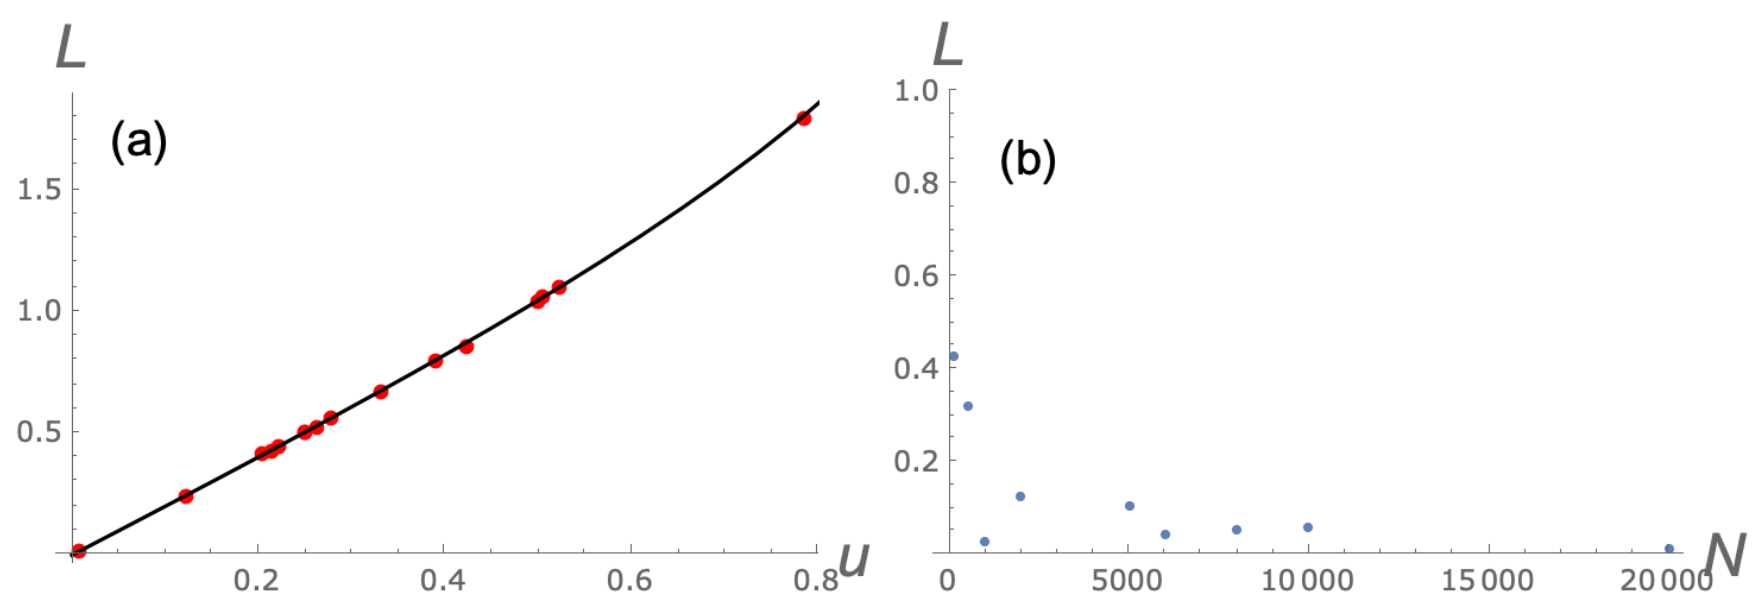
\includegraphics[width=0.9\textwidth]{fig6.png}
        \end{figure}
    $$
    \Gamma(\xi, \eta) = \sin\xi + u\sin \eta = 0
    $$
    where $u:=U_-/U_+$

\end{frame}

% -----------------------------------------------------------------------------
\end{document}